%%% Local Variables:
%%% mode: latex
%%% TeX-master: "../main"
%%% End:

\part{Results and Experiments}

\begin{figure}[H]
  \centering
  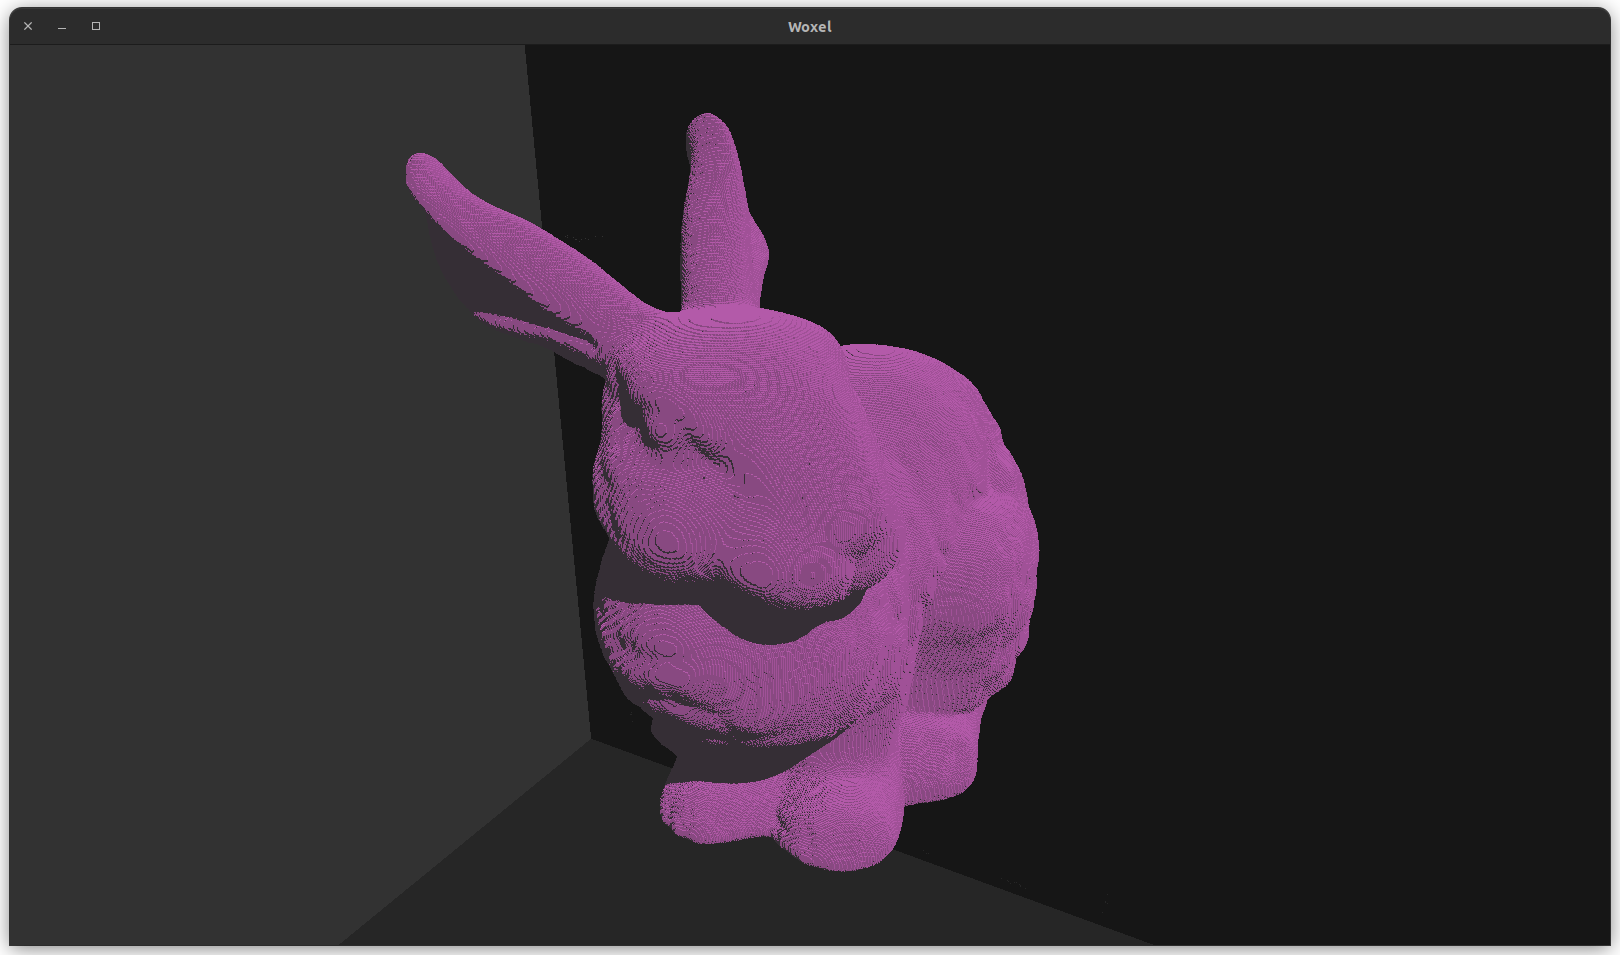
\includegraphics[width=0.8\textwidth]{bunny}
  \caption{Bunny with diffuse pink material, model voxel resolution: $628\times621\times489$}
\end{figure}

\section{Images}

This section shows some images captured in the rendering engine. All the models used are samples from the OpenVDB website\supercite{openvdb:models}. Each of the figures bellow showcase a different functionalities of the engine.

\begin{figure}[H]
  \centering
  \begin{subfigure}[b]{0.48\textwidth}
    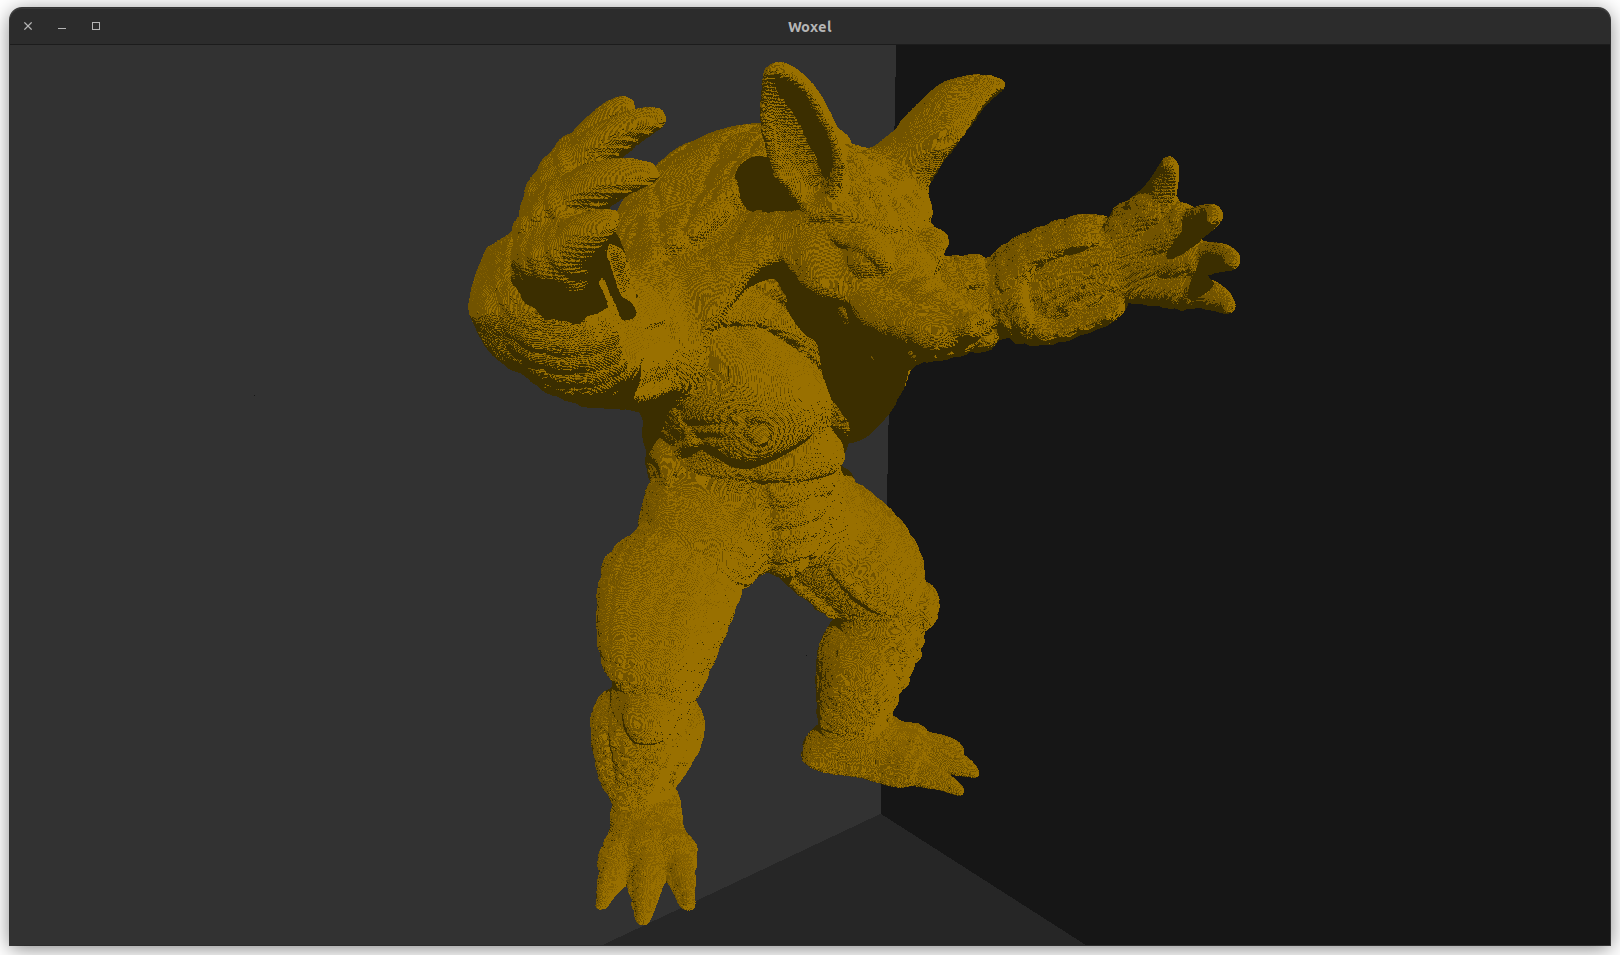
\includegraphics[width=\textwidth]{arm_1}
  \end{subfigure}
  \hfill
  \begin{subfigure}[b]{0.48\textwidth}
    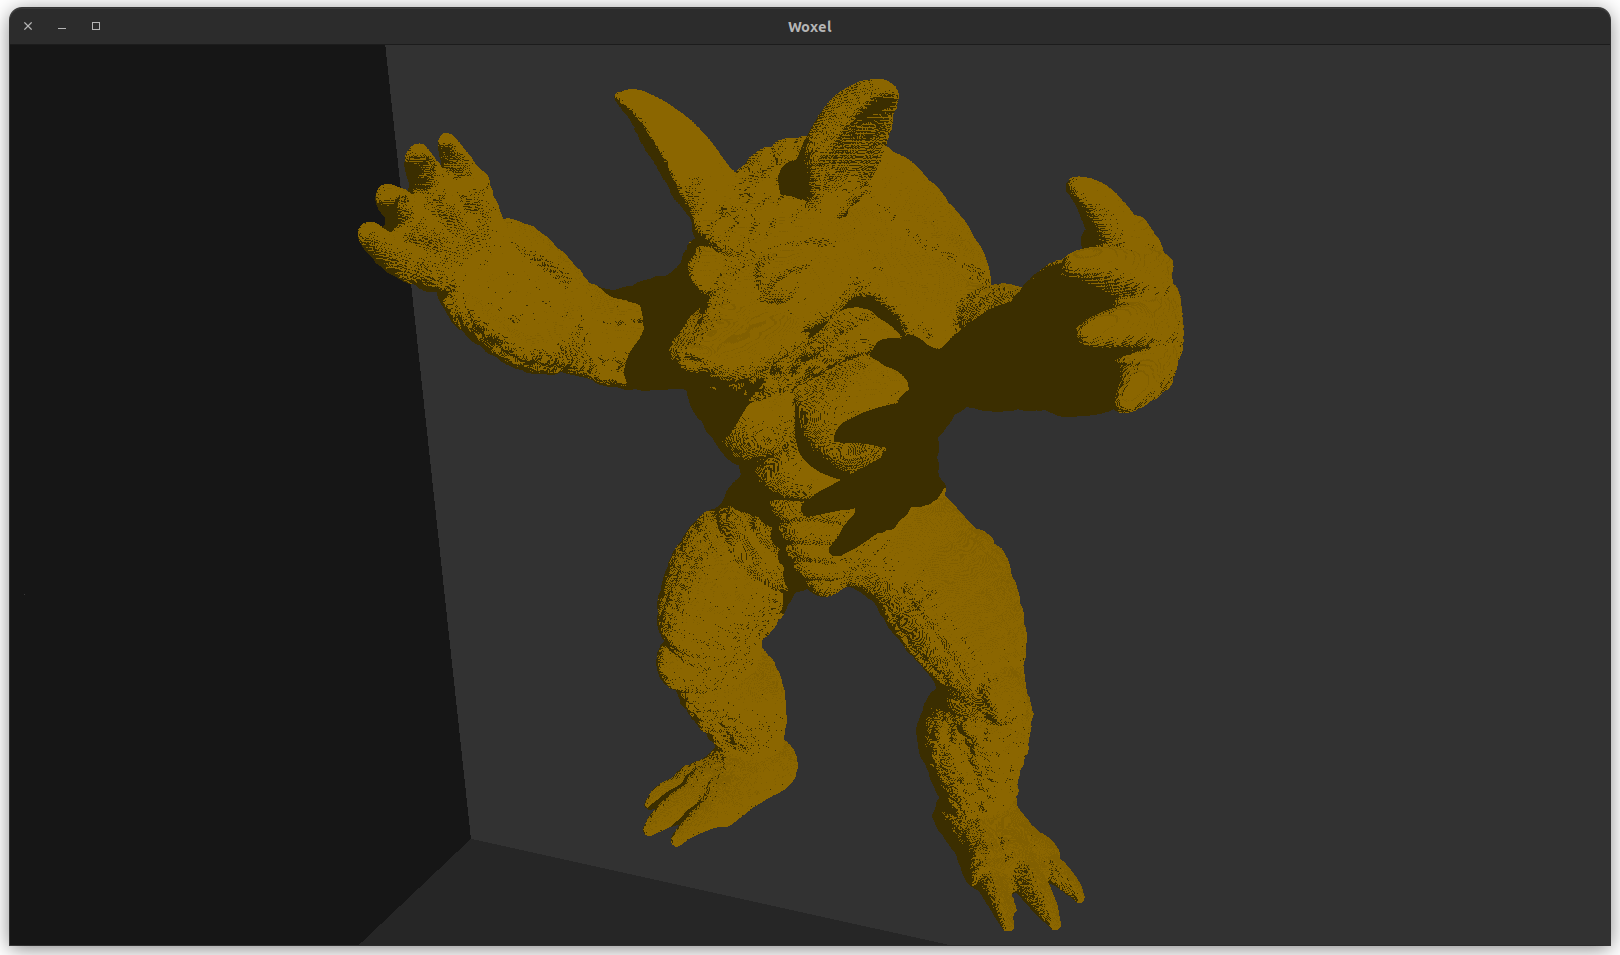
\includegraphics[width=\textwidth]{arm_2}
  \end{subfigure}
  \begin{subfigure}[b]{0.48\textwidth}
    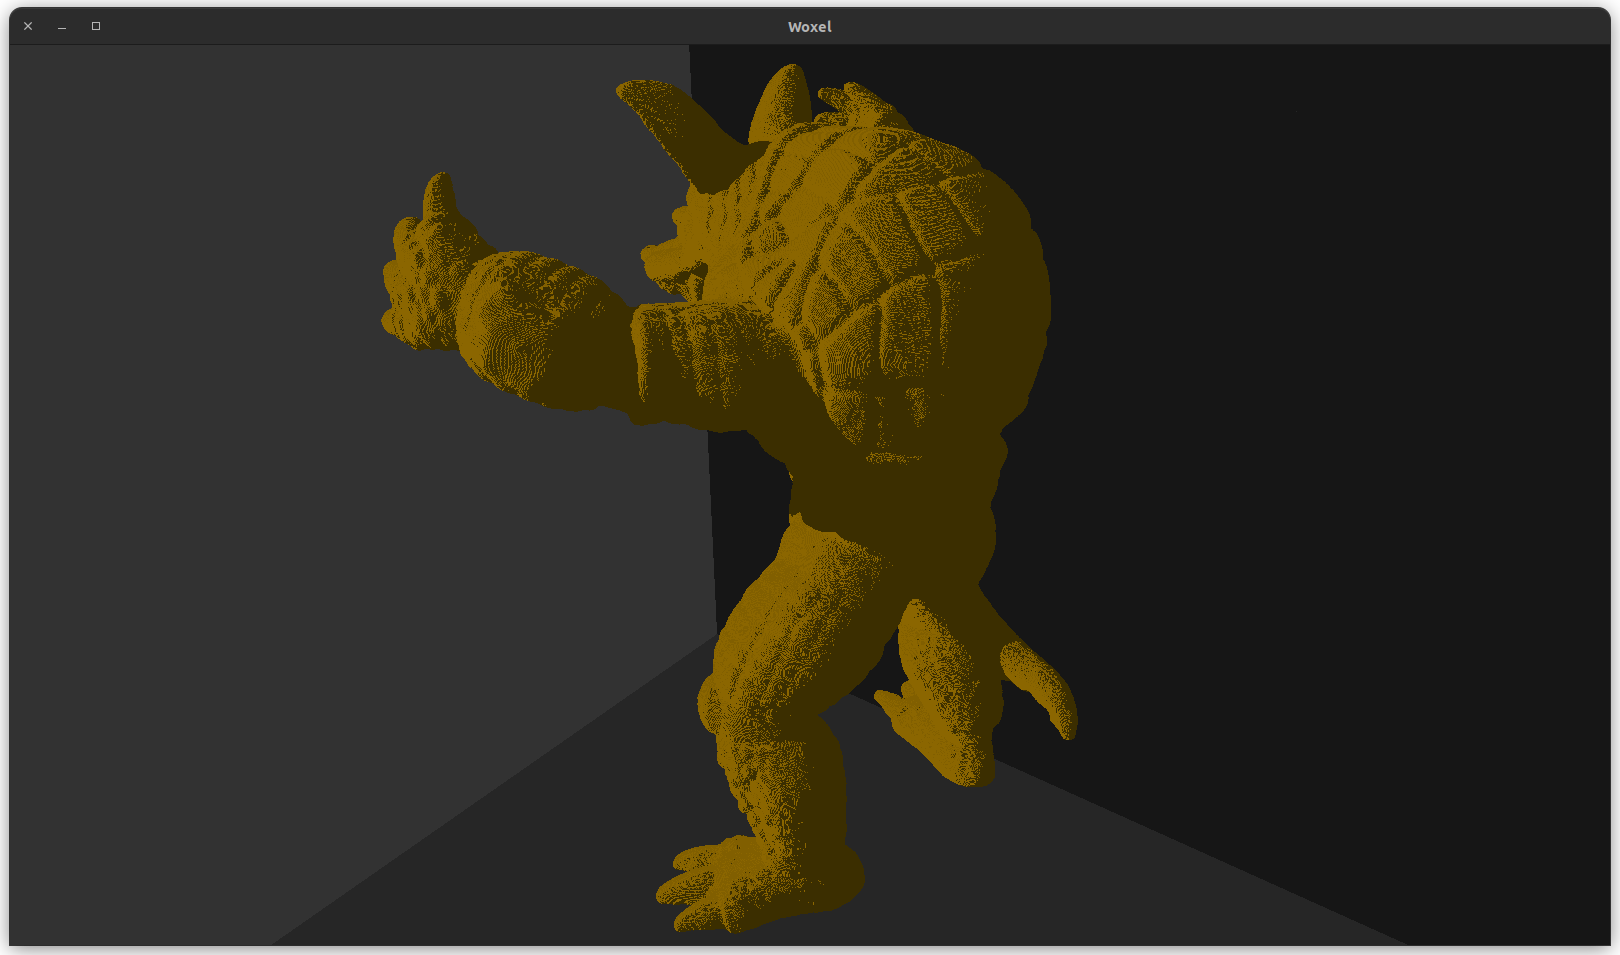
\includegraphics[width=\textwidth]{arm_3}
  \end{subfigure}
  \hfill
  \begin{subfigure}[b]{0.48\textwidth}
    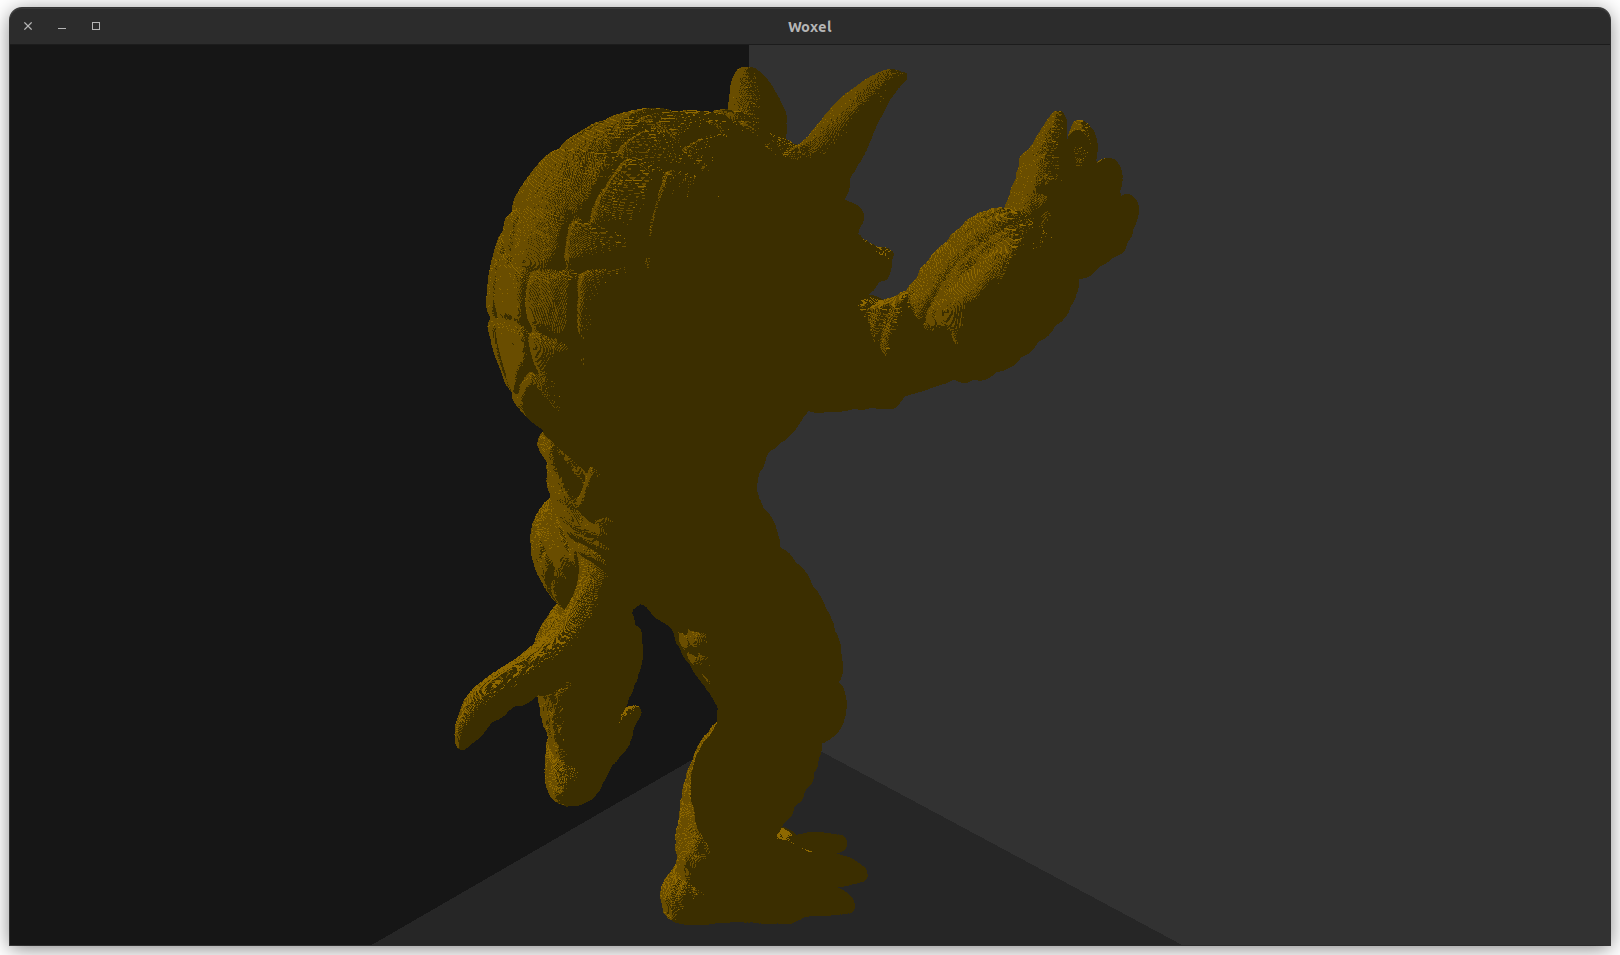
\includegraphics[width=\textwidth]{arm_4}
  \end{subfigure}
  \caption{\textbf{Multiple angles} of an armadilo model with a diffuse material. The voxel resolution of the model is $1276\times1518\times116$}
\end{figure}

\begin{figure}[H]
  \centering
  \begin{subfigure}[b]{0.48\textwidth}
    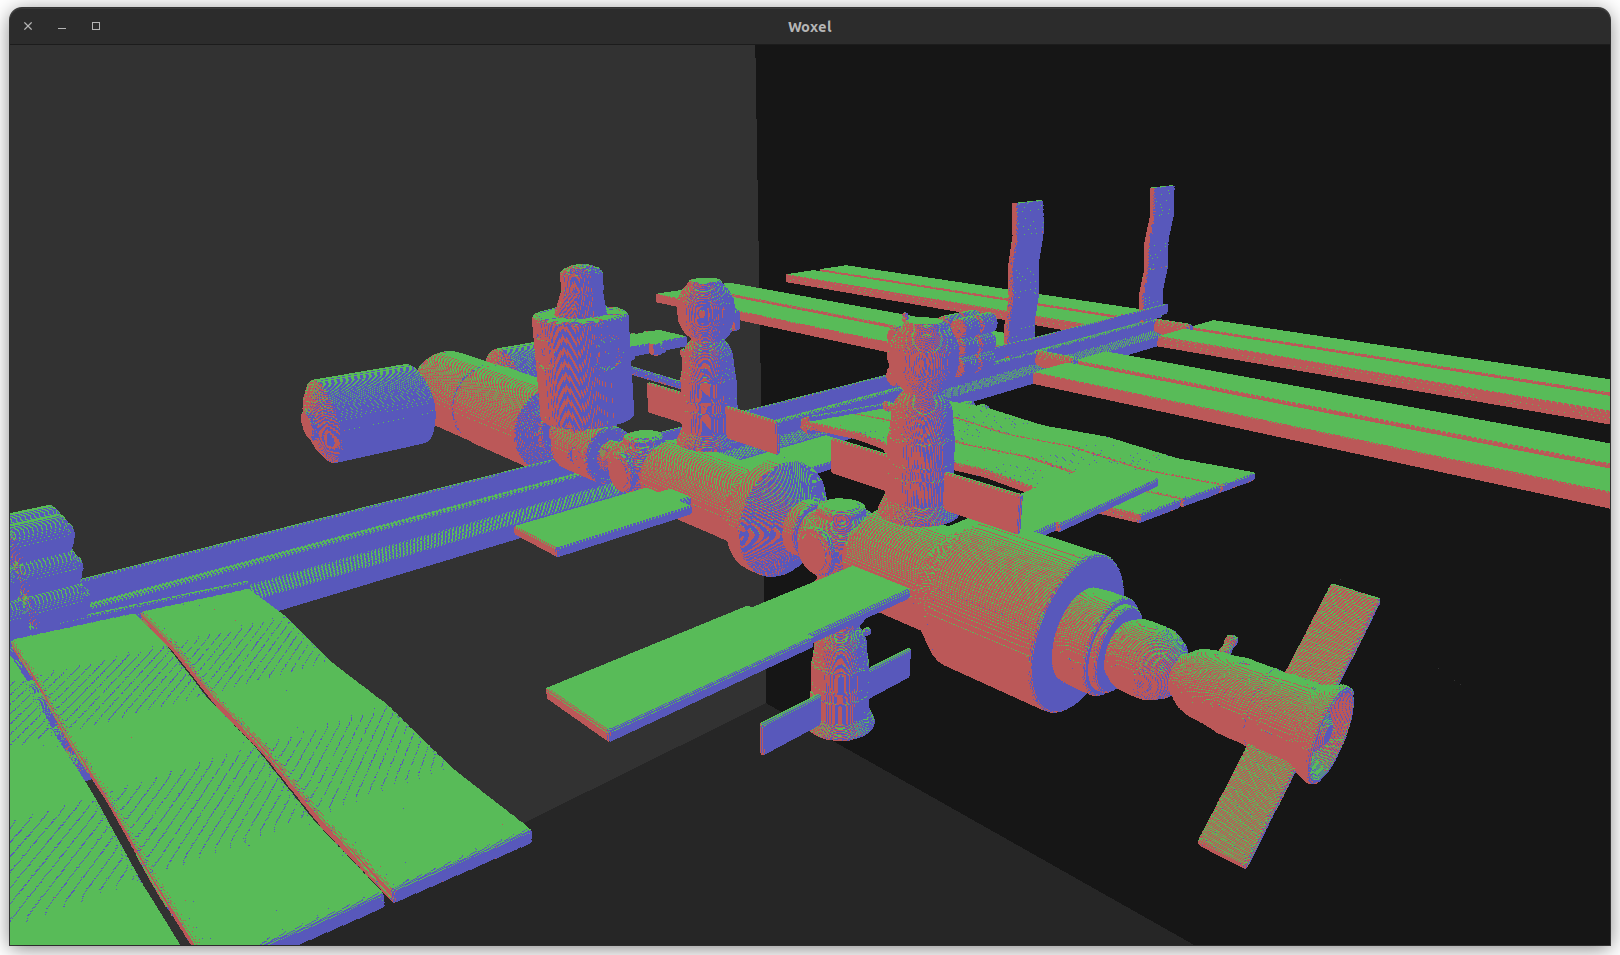
\includegraphics[width=\textwidth]{iss_rgb}
    \caption{RGB}
  \end{subfigure}
  \hfill
  \begin{subfigure}[b]{0.48\textwidth}
    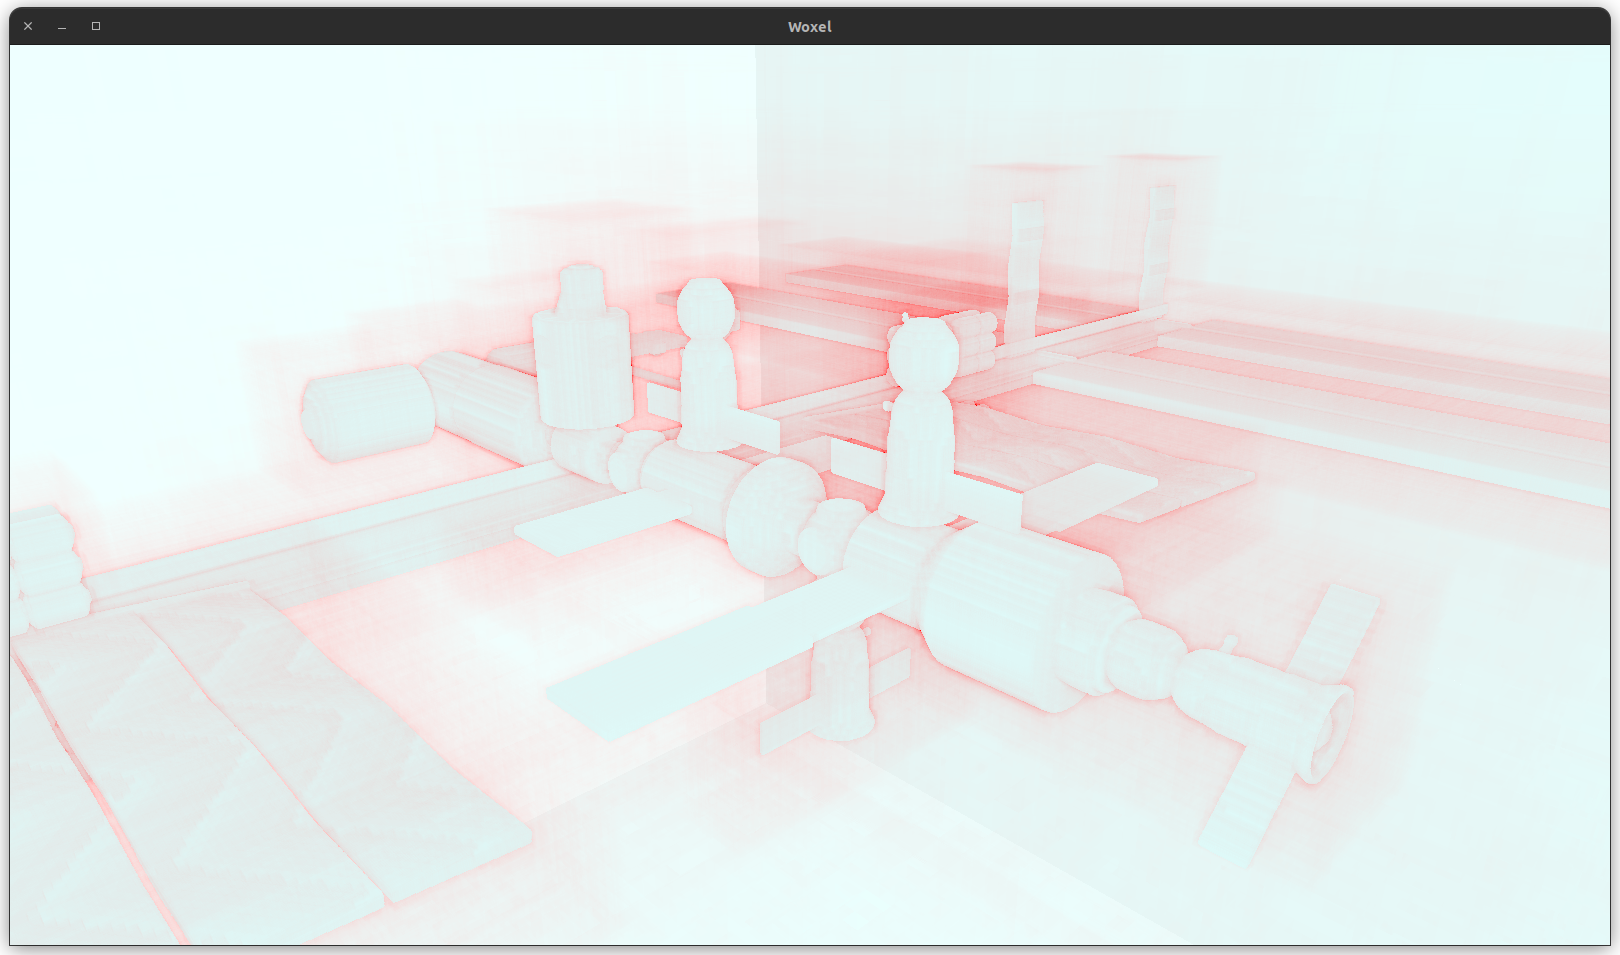
\includegraphics[width=\textwidth]{iss_ray}
    \caption{Ray}
  \end{subfigure}
  \begin{subfigure}[b]{0.48\textwidth}
    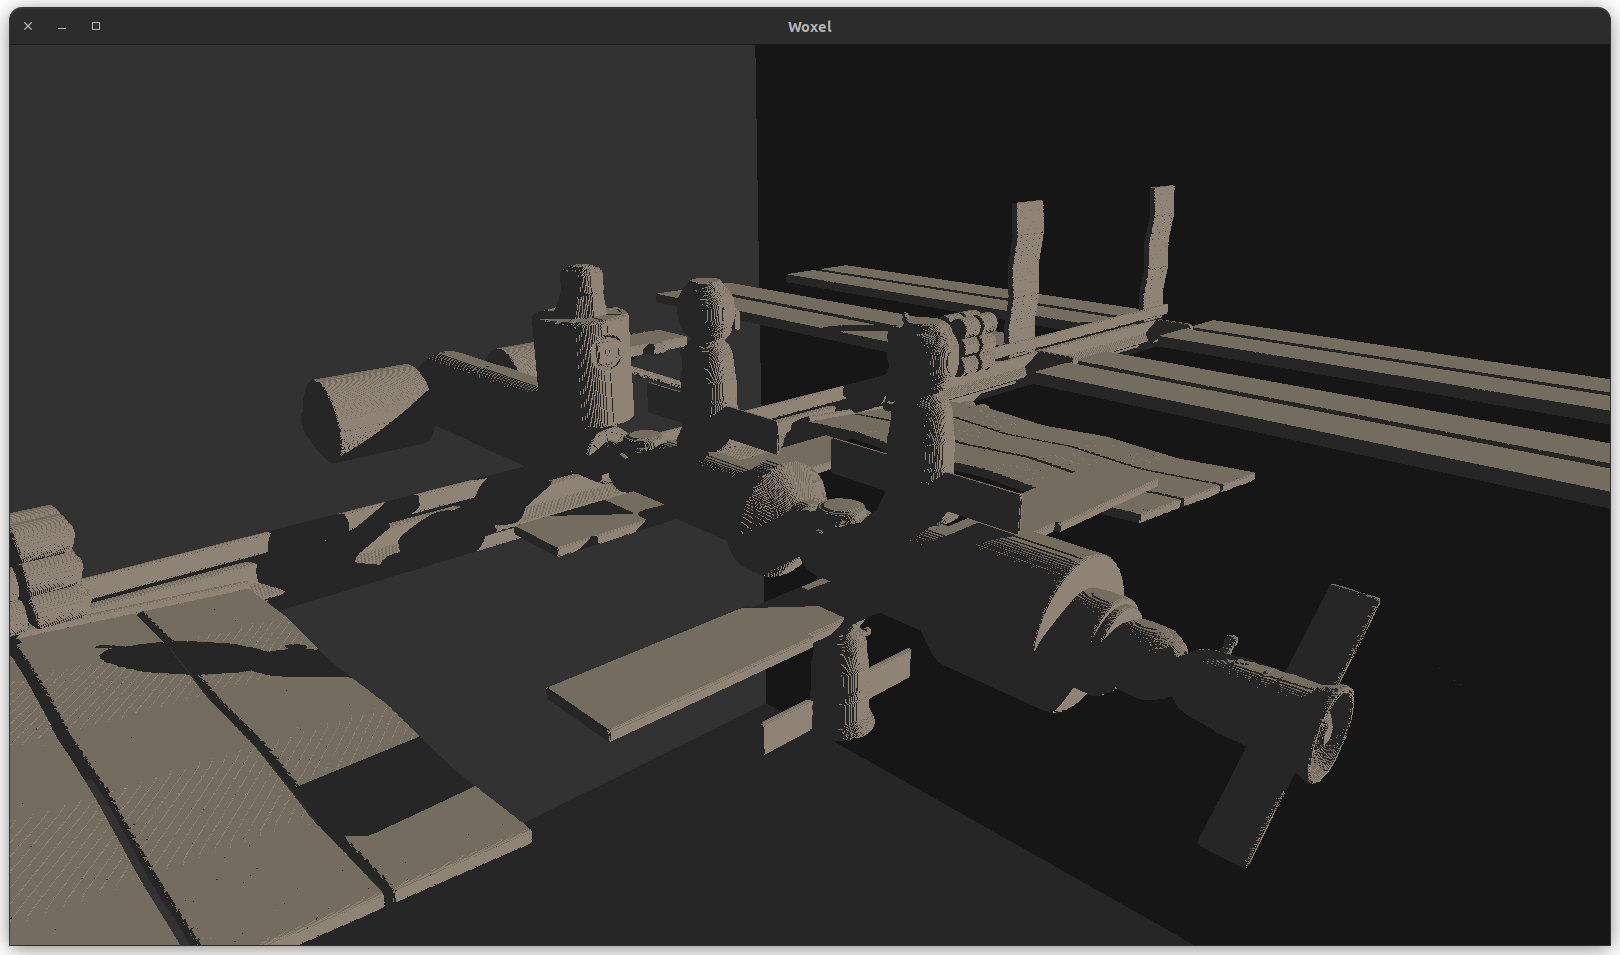
\includegraphics[width=\textwidth]{iss_diffuse}
    \caption{Diffuse}
  \end{subfigure}
  \hfill
  \begin{subfigure}[b]{0.48\textwidth}
    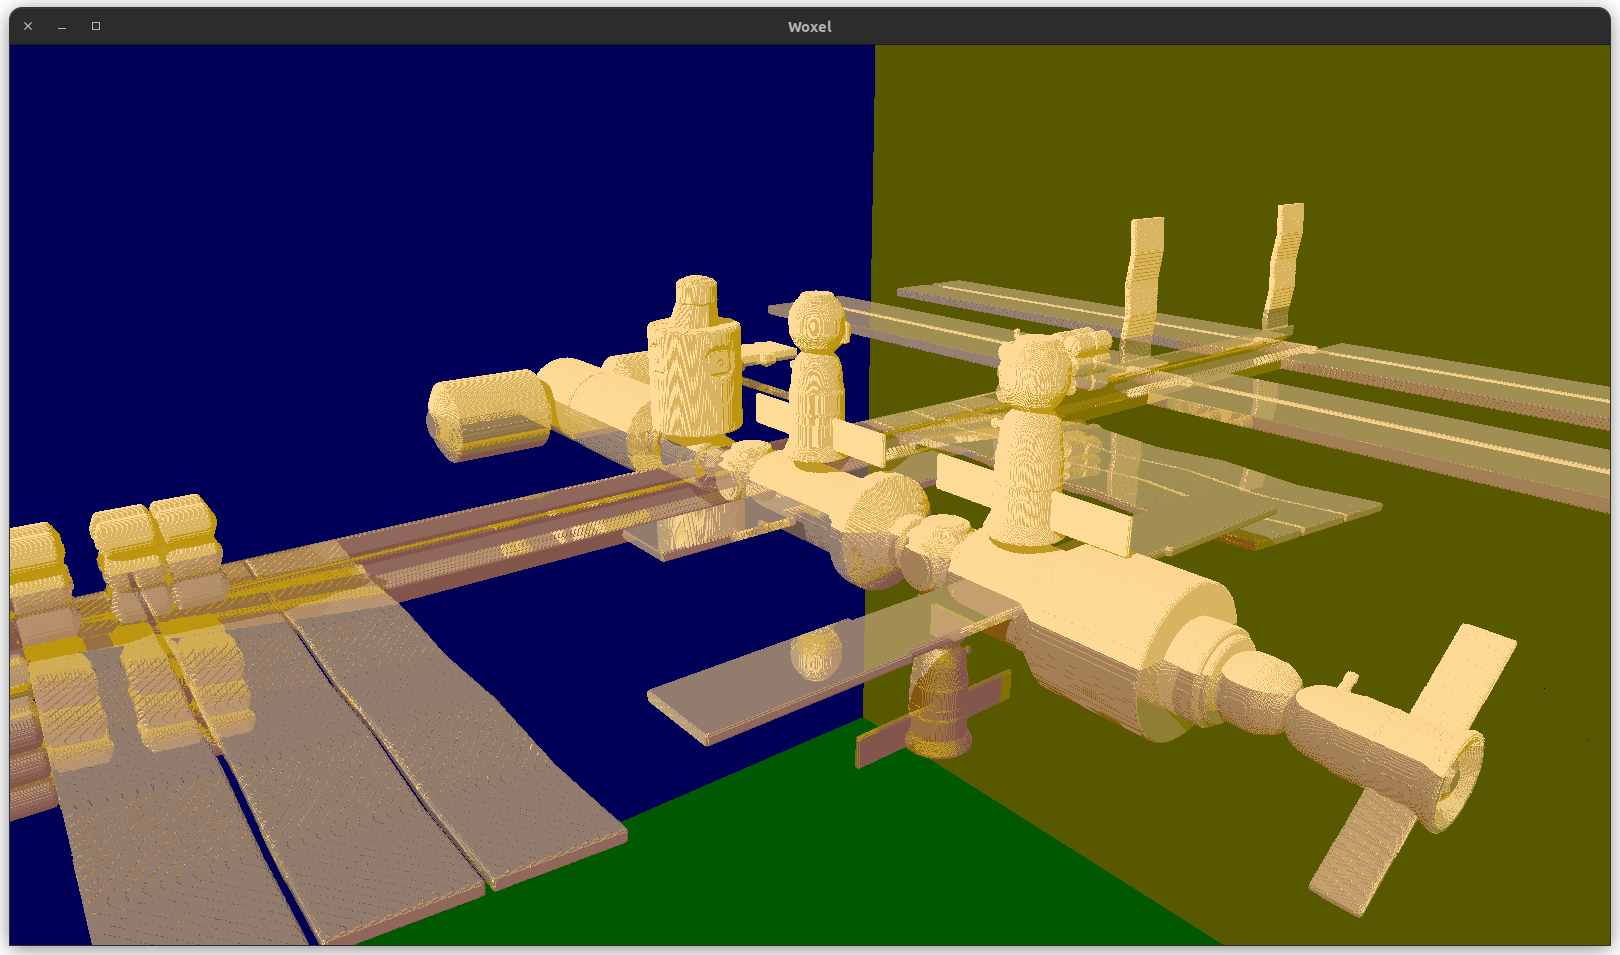
\includegraphics[width=\textwidth]{iss_gloss}
    \caption{Glossy}
  \end{subfigure}
  \caption{\textbf{Render modes} on a ISS model with voxel resolution $4561\times617\times2999$
    (a): RGB mode colors each face based on what axis it is parallel to.
    (b): Ray mode colors each pixel based on how many steps the ray took. The color is interpolated between light blue and red based on how many steps the ray took to go out of bounds or intersect a voxel. Maximum (red) is 200 steps.
    (c): Diffuse mode shows an object with diffuse material lit by sunlight.
    (d): Glossy mode shows a half glossy (bottom), half diffuse (top) model lit by sunlight. The out of bounds box is colored to discriminate which is face reflected on what surface. The reflection of the middle pod with a sphear on top can be seen in the solar panel in the middle. More reflections can be seen in the solar panels one the left and right.
  }
  \label{rendermods}
\end{figure}


\begin{figure}[H]
  \centering
  \begin{subfigure}[b]{0.48\textwidth}
    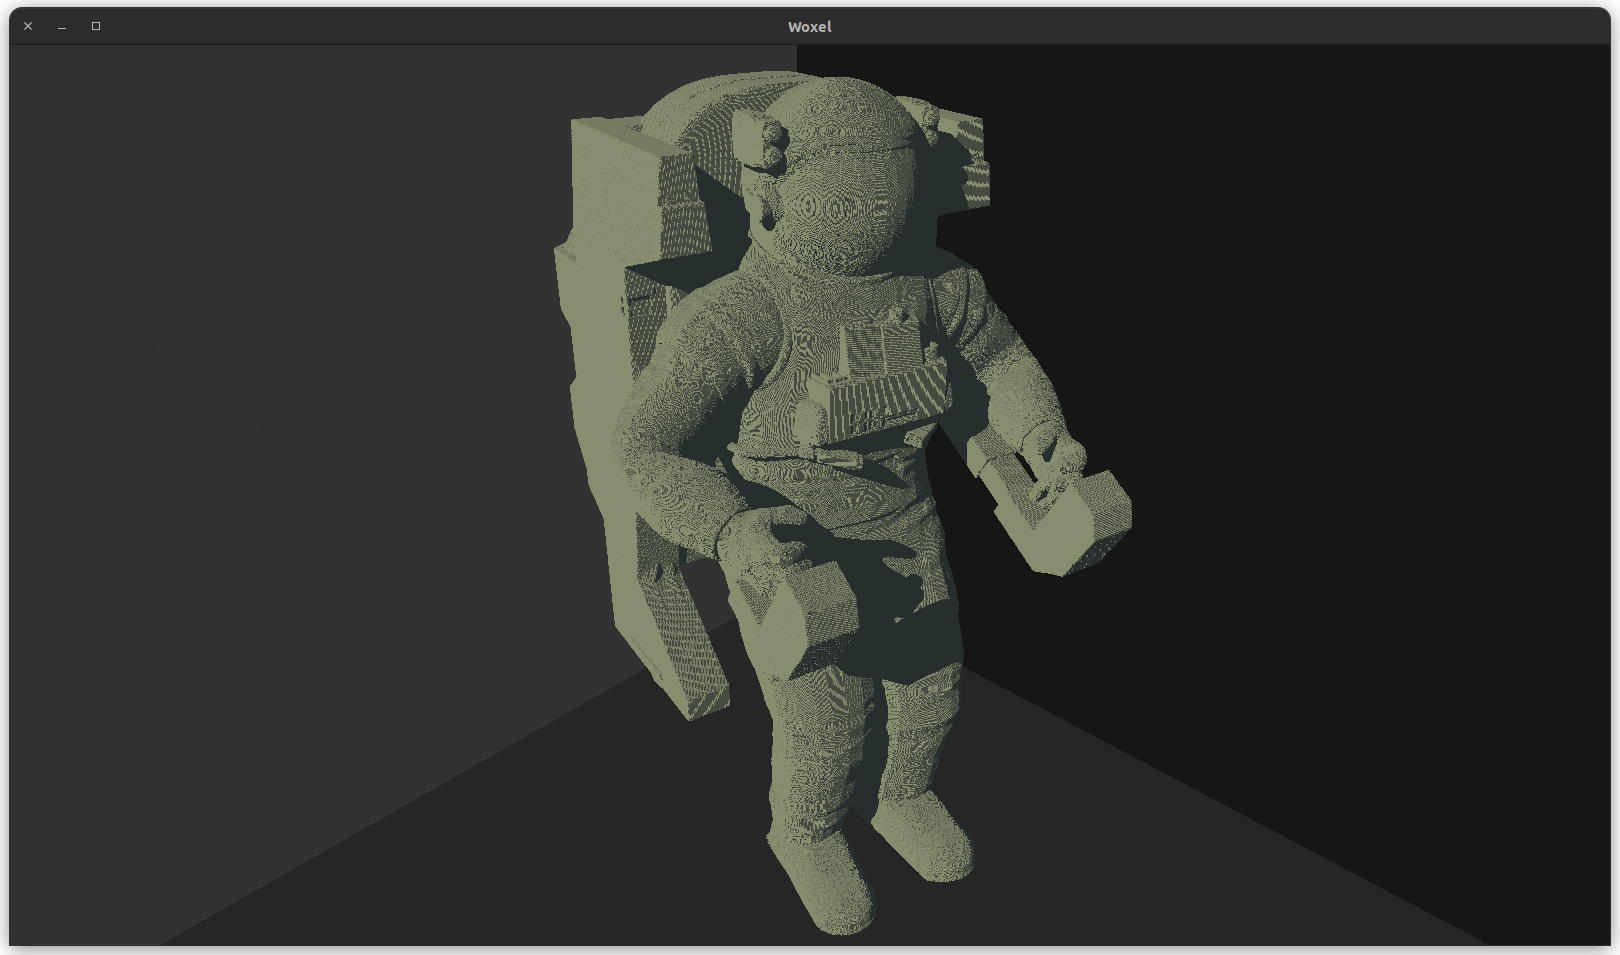
\includegraphics[width=\textwidth]{astro_1}
  \end{subfigure}
  \hfill
  \begin{subfigure}[b]{0.48\textwidth}
    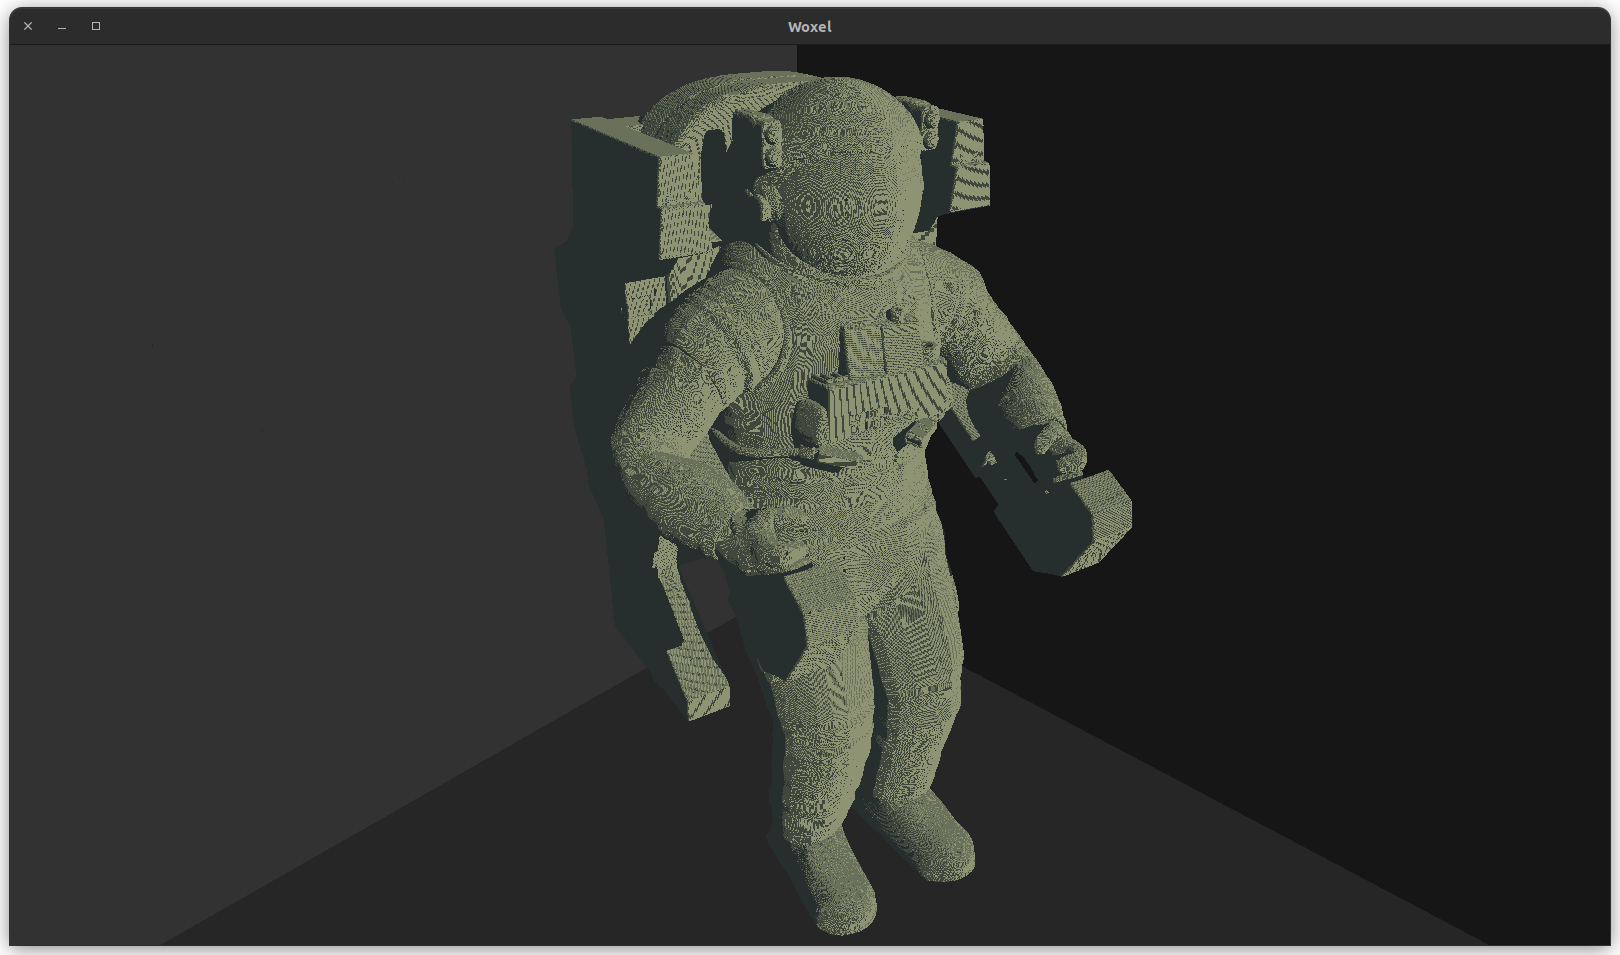
\includegraphics[width=\textwidth]{astro_2}
  \end{subfigure}
  \begin{subfigure}[b]{0.48\textwidth}
    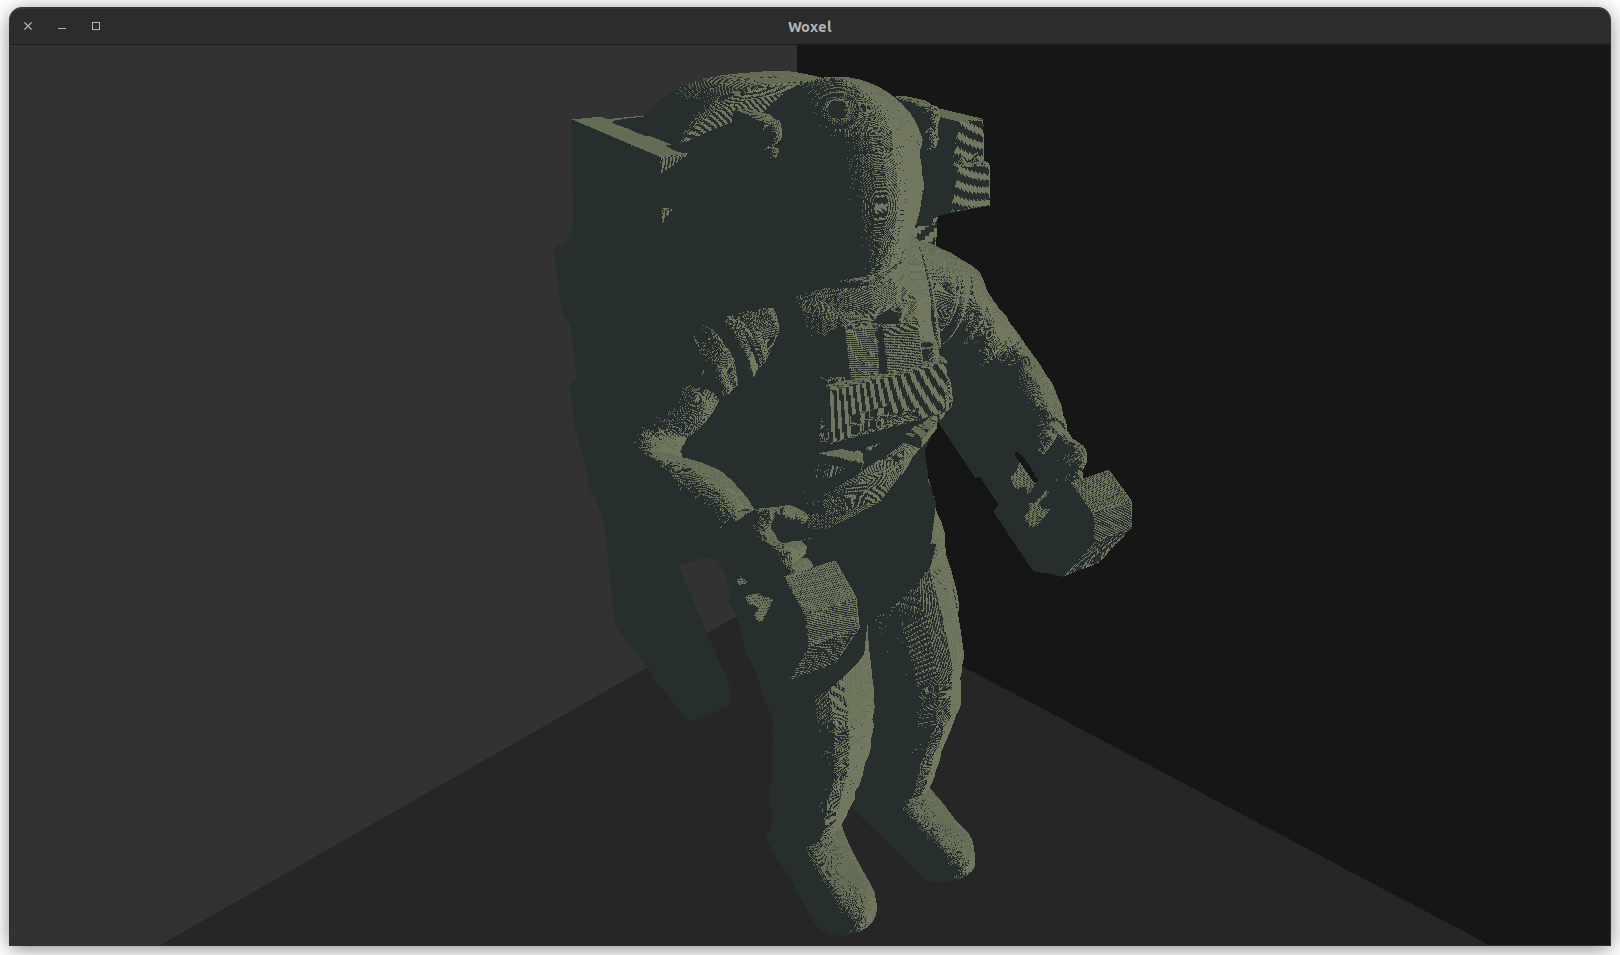
\includegraphics[width=\textwidth]{astro_3}
  \end{subfigure}
  \hfill
  \begin{subfigure}[b]{0.48\textwidth}
    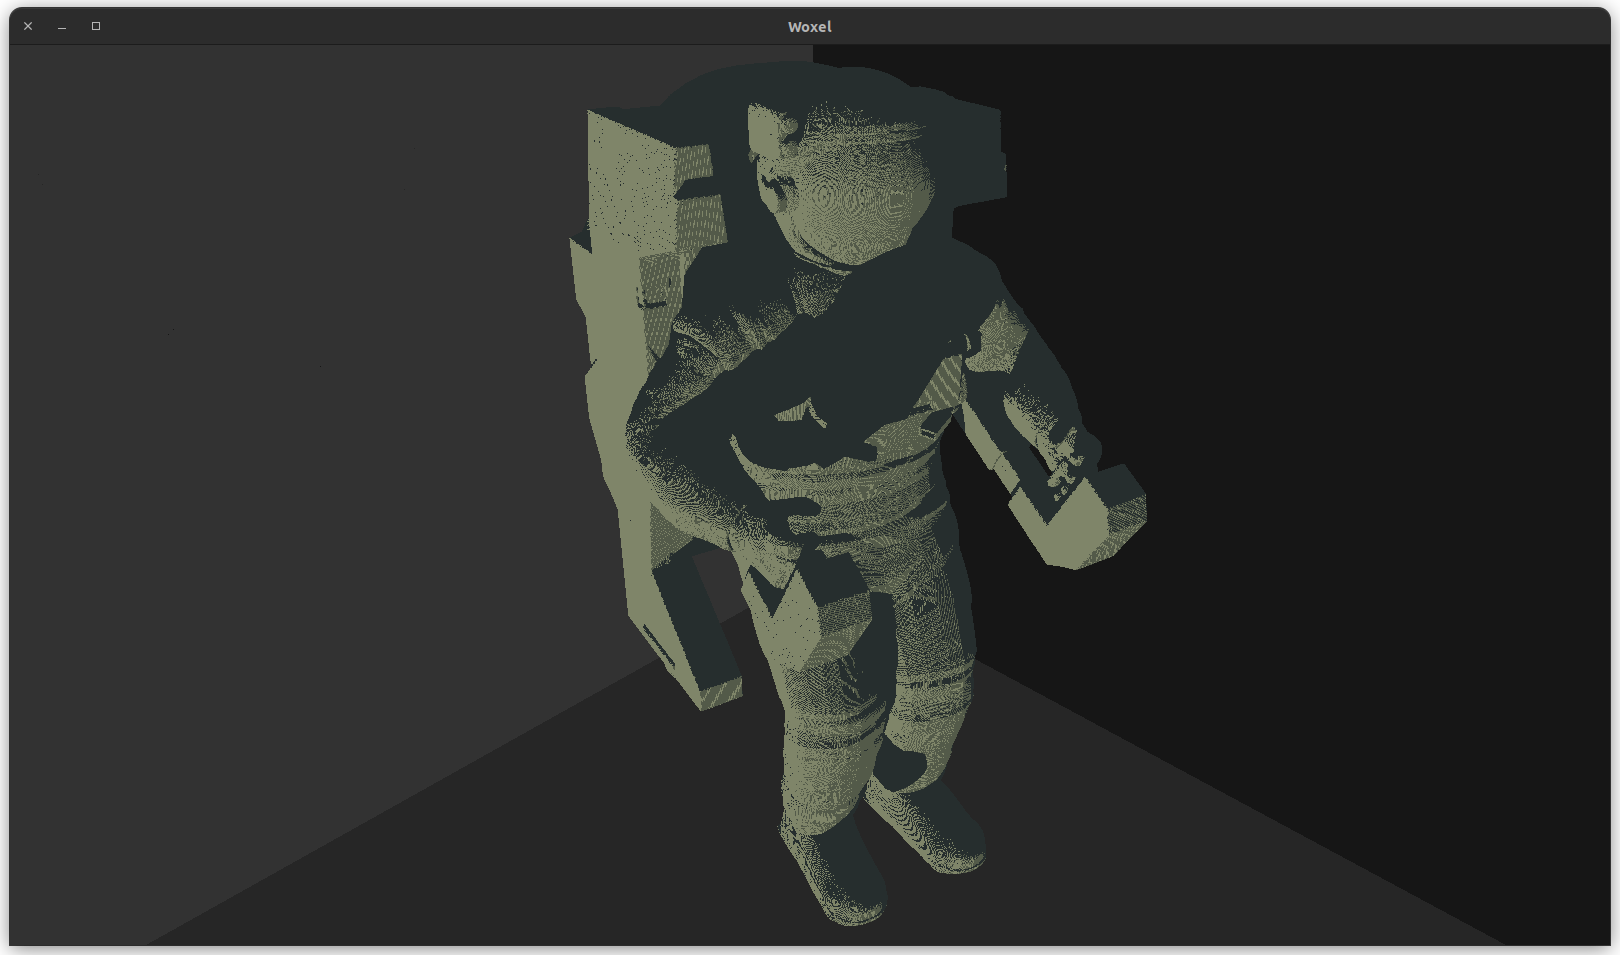
\includegraphics[width=\textwidth]{astro_4}
  \end{subfigure}
  \caption{\textbf{Dynamic Lighting} on an astronaut model. The sunlight is dynmaic, its direction, color and intensity can be changed through the developer GUI in real-time. The voxel resolution of the model is $1481\times2609\times1843$}
\end{figure}

\begin{figure}[H]
  \centering
  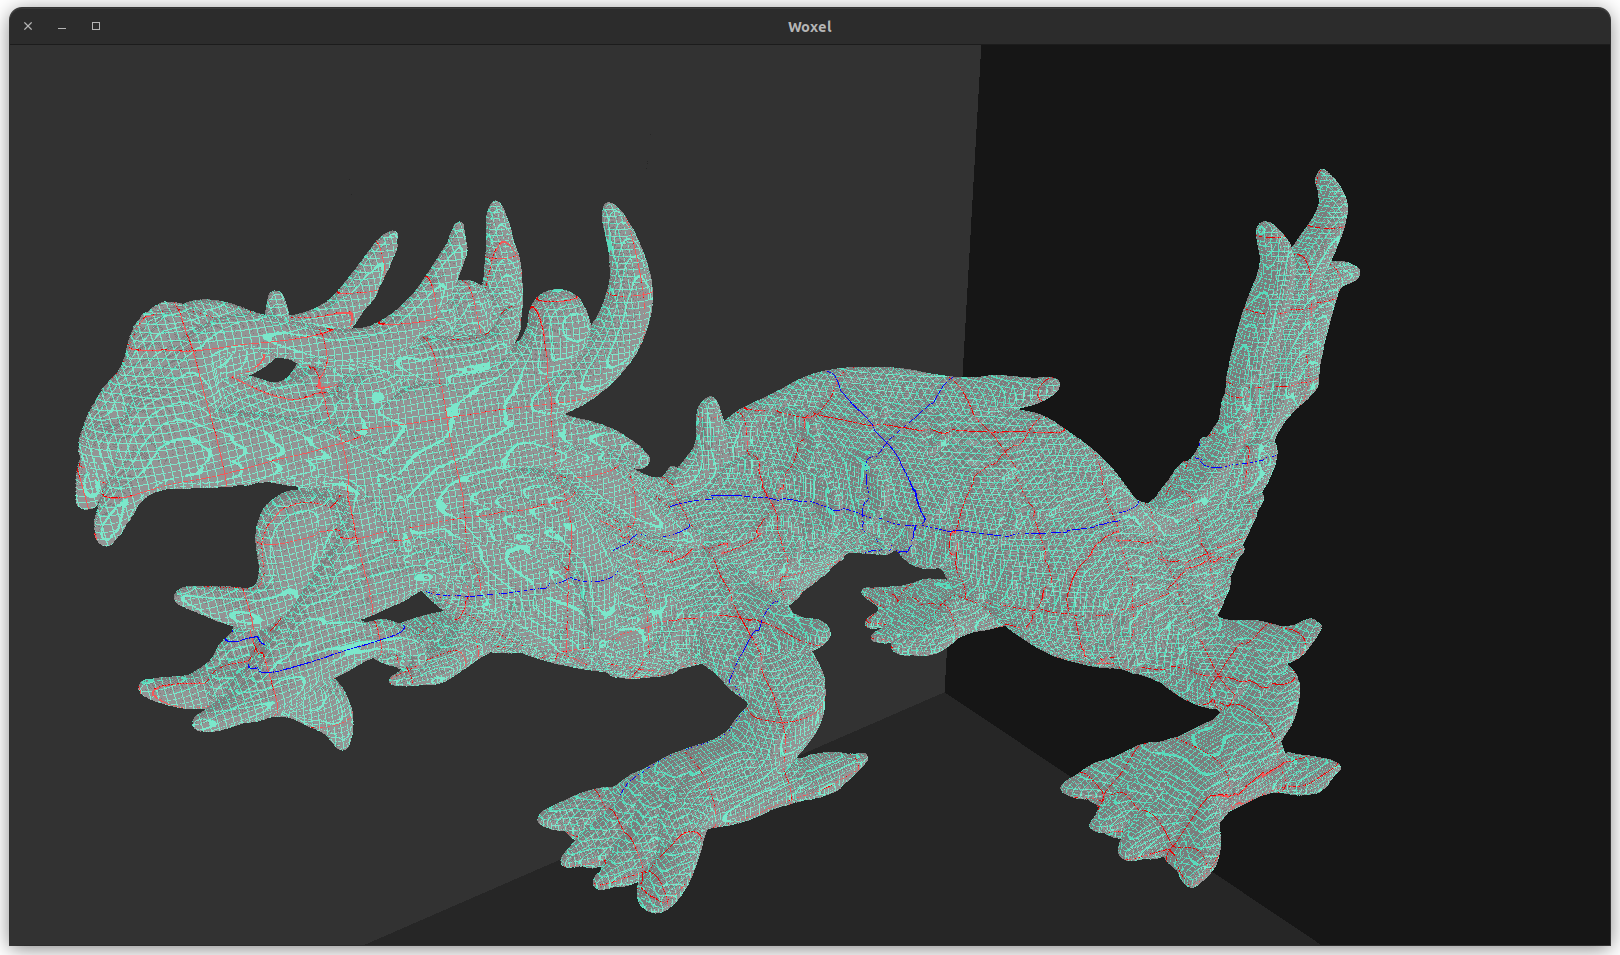
\includegraphics[width=0.8\textwidth]{dragon_3}
  \caption{\textbf{VDB highligthing}: Voxels at the boundries of VDB nodes are highlighted on a dragon model. The grid structure of the VDB can be seen at each level in the hierarchy. Node3, Node4 and Node5 boundries are shown in Cyan, Red and Blue respectively. The voxel resolution of the model is $2023\times911\times1347$}
\end{figure}

\begin{multicols}{2}[]
  \begin{figure}[H]
    \centering
    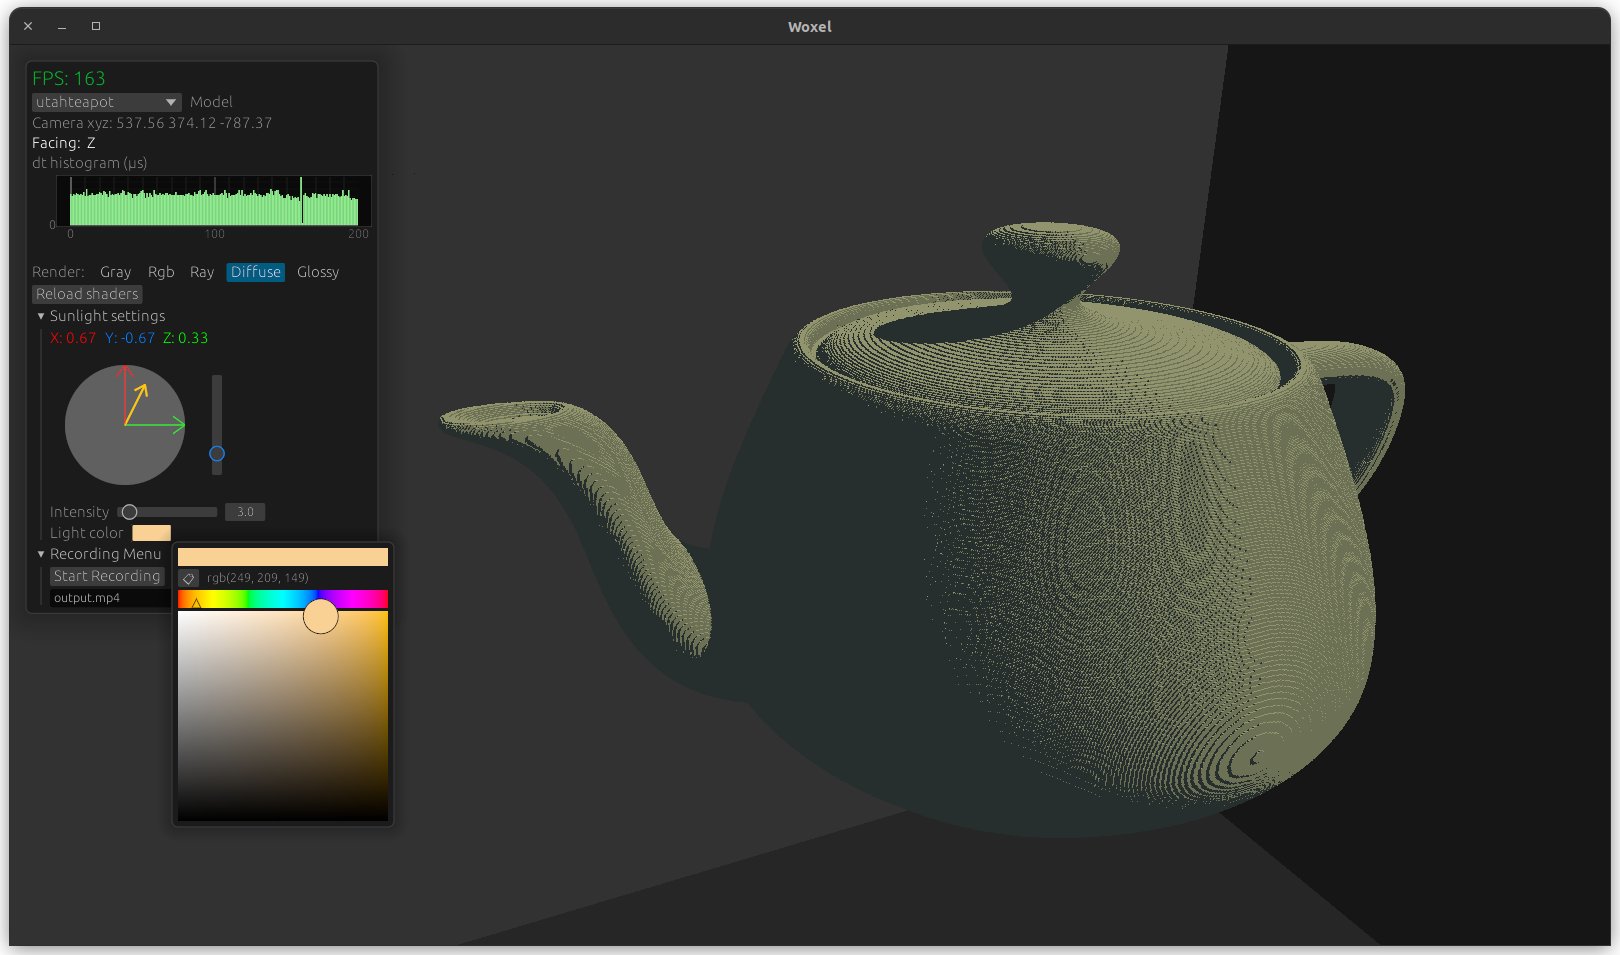
\includegraphics[width=0.96\linewidth]{gui_1}
    \caption{Developer GUI in engine}
  \end{figure}
  The developer GUI has the following uses:
  \begin{enumerate}[itemstep=0mm]
    \item Display current \acrshort{FPS} and histogram of milliseconds per frame.
    \item Changing the model in the viewport through a drop down menu that scans the assets folder for available models.
    \item Camera coordinates and facing direction
    \item Functionality to change between the render modes presented in \cref{rendermods}
    \item The option to reload the shaders while the engine is running.
    \item For the diffuse and glossy render modes there is a sunlight section available.
    \item The recording menu allows setting an output file and starting or ending the recording.
  \end{enumerate}
  \columnbreak
  \begin{figure}[H]
    \centering
    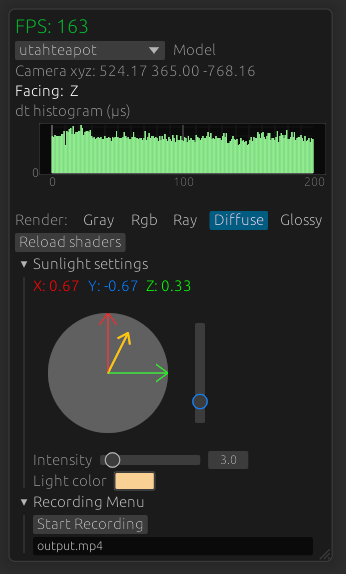
\includegraphics[width=1.0\linewidth]{gui_2}
    \caption{Developer GUI close-up}
    \label{gui}
  \end{figure}
\end{multicols}

\section{Benchmarks}
In this section the ray catsing algorithms are compared against each other on different models and render modes.

The specifications of the machine the experiments where ran on are presented in \cref{specs}.
\begin{table}[h]
  \centering
\begin{tabular}{|c||c|}
  \hline
  \multicolumn{2}{|c|}{Experiment machine specifications} \\
  \hline
  OS & Ubuntu 22.04.3 LTS x86\_64\\
  \hline
  CPU & AMD Ryzen 7 5800H with Radeon\\
  \hline
  GPU &  NVIDIA GeForce RTX 3070 Mobile\\
  \hline
  RAM & 8192MiB \\
  \hline
  FMA & Enabled \\
  \hline
\end{tabular}
  \caption{Experiment machine specifications}
  \label{specs}
\end{table}

\subsection{Comparing DDA, HDDA and HDDA+SDF}

First the average millseconds per frame are compared for the DDA, HDDA and HDDA+SDF algorithms is compared on the teapot model at 3 distinct distances from the model, one further a way, ore closer and one near the model.

\begin{table}[h]
  \centering
  \begin{tabular}{|c||c|c|c|}
    \hline
    & 2000m & 1000m & 500m \\
    \hline
    DDA & 100ms* & 100ms* & 50ms \\
    \hline
    HDDA & 9.4ms & 12.5ms & 14.4ms \\
    \hline
    HDDA & 9.4ms & 12.5ms & 14.4ms \\
    \hline
    HDDA+SDF & 6ms** & 6.4ms & 7.6ms\\
    \hline
  \end{tabular}
  \caption{Milliseconds per frame of rendering the teapot model using DDA, HDDA, HDDA+SDF at far, medium, and close distance. A voxel is considered $1\rm{m}\times1\rm{m}\time1\rm{m}$. (*): Model doesn't show in viewport because the algoirhtm exceeds the maximum step size. This time can be treated as the wors-case scenario, casting bouncing the maximum number of times for each pixel. (**): Frame rate cap is hit at 165 FPS}
\end{table}

\section{Future work}
\section{Final remarks}
